
% POSTER EXAMPLE
%
% This is an example of a relatively sane poster. The box structure (and the
% narrative in general) is what I would expect, but it is completely
% non-mandatory; you may include whatever you want. Preferably, erase the
% existing box structure after you read it, and start from scratch.
%
% The main communication requirements for the poster that should be satisfied
% are as such:
%
% - At the defense, it should help you talk for around 10 minutes about your
%   thesis, and convince the committee that you did something interesting and
%   sufficiently complicated. Prepare pictures that explain your main results.
%
% - It should quickly communicate the main idea of your thesis to a random
%   educated by-walker. Ideally, a moderately-witted MFF graduate who has never
%   heard about your thesis before should be able to get the main "rough idea"
%   in less than 1 minute by just looking at the poster.

% modify the fontscale parameter to make everything slighly bigger or smaller.
\documentclass[portrait,a0paper,fontscale=0.25]{baposter}

\usepackage[utf8]{inputenc}
\usepackage[T1]{fontenc}

% FONT CHOICES
% Posters do not need to be PDF/A; you can choose any relatable font from the
% TeX font catalogue without much risk. Sans-serif fonts are suggested for the
% posters; see https://tug.org/FontCatalogue/sansseriffonts.html
\usepackage[sfdefault]{Fira Sans}
%\usepackage[default]{droidsans}
%\usepackage[math]{iwona}
%\usepackage[defaultfam]{montserrat}
%\usepackage{cmbright}
%\usepackage{yfonts}\renewcommand{\familydefault}{\frakdefault}

\usepackage{color}
\usepackage{graphicx}
\usepackage{amssymb,amsmath}
\usepackage[export]{adjustbox} %allows using valign with \includegraphics

\renewcommand{\arraystretch}{1.5}

\usetikzlibrary{positioning}

% A WORD ABOUT COLORS
%
% This template is prepared with a relatively neutral gray background that
% gives decent box borders (with white and darker gray), does not clash with
% many colors (except for violet-brown and other mushroomish colors, perhaps)
% and gives a lot of space for highlighting stuff.
%
% Generally, other color variations are good too; there are no strict rules on
% the colors. Good choices include:
%
% - white backgrounds and differentiation of box headers by color (see
%   headerFontColor)
%
% - various slightly tinted backgrounds (try red!10 instead of black!3)
% 
% - dark backgrounds
%
% Keep in mind:
% - The normal "informative" text and figures should be DARK on LIGHT
%   background, not the other way around.
%
% - If you want a dark background, soften (darken) the box backgrounds a bit so
%   that they do not "shine" too much from the poster. Use \color{white} for
%   the heading, and switch the UK/MFF logos to white (see contents of logos/).
%
% - Do not mix too many color hues together. Most hues have their widely
%   accepted meaning (green: good result, red: problem, blue: information,
%   yellow: highlighter, brown: serious problem, violet: something really
%   weird/interesting/magic, depending on the shade).

\begin{document}

\color{black!80} % default font color
\begin{poster}{grid=false,
	eyecatcher=true,
	background=plain,
	bgColorOne=black!3, % background color
	columns=2,
	headerborder=none,
	textborder=none,
	headershape=rectangle,
	headershade=plain,
	boxshade=plain,
	boxColorOne=white,
	headershade=plain,
	headerColorOne=black!15, % box header background color
	headerFontColor=black,
	}%
	{
\includegraphics[height=7em]{logos/mff-black.pdf}}
	{Extension of web-based interface for protein binding sites prediction}
	{\vspace{1ex} Lukáš Polák}
	{
\includegraphics[height=7em]{logos/uk-red.pdf}}


%
% LEFT COLUMN
%

\begin{posterbox}[column=0,name=intro]{Introduction}

Lorem ipsum dolor sit amet, consectetur adipiscing elit. Sed euismod, nisl quis
consequat ultricies, nunc ipsum aliquam nunc, vitae aliquam nisl nunc eu
nunc. Nulla facilisi. Nulla facilisi. Nulla facilisi. Nulla facilisi.

\begin{center}
\begin{tikzpicture}[ultra thick, inner sep=1ex]
\node[rectangle, rounded corners=1ex, draw=red!80!black, color=red!80!black, font=\huge\bfseries, rotate=21] {Problem!};
\end{tikzpicture}\end{center}
\end{posterbox}

\begin{posterbox}[column=0, name=goals, below=intro, headerColorOne=cyan!60, boxColorOne=cyan!20]{Thesis goals}
There were two main goals of the thesis:
\begin{itemize}
\item Improve the web frontend, replace old and unsupported components with new ones.
\item Extend the server architecture to enable simple addition of modules for postprocessing of the predicted
binding sites.
\end{itemize}
\end{posterbox}

\begin{posterbox}[column=0, name=architecture, below=goals]{Server architecture}

This box will contain a description of the server architecture \dots

This box may contain an overview of the used methods, mathematics, program structure, etc.

Include a picture, because pictures are better. Thesis defense takes less than 10 minutes, no one can read a wall of text in that short time. (For comparison, the usual realistic poster visit on a conference takes 15 seconds, unless the poster manages to catch the attention in that short time.)

TODO: add a diagram of the server architecture

Lorem ipsum dolor sit amet, consectetur adipiscing elit. Sed euismod, nisl quis
consequat ultricies, nunc ipsum aliquam nunc, vitae aliquam nisl nunc eu
nunc. Nulla facilisi. Nulla facilisi. Nulla facilisi. Nulla facilisi.

Lorem ipsum dolor sit amet, consectetur adipiscing elit. Sed euismod, nisl quis
consequat ultricies, nunc ipsum aliquam nunc, vitae aliquam nisl nunc eu
nunc. Nulla facilisi. Nulla facilisi. Nulla facilisi. Nulla facilisi.

Lorem ipsum dolor sit amet, consectetur adipiscing elit. Sed euismod, nisl quis
consequat ultricies, nunc ipsum aliquam nunc, vitae aliquam nisl nunc eu
nunc. Nulla facilisi. Nulla facilisi. Nulla facilisi. Nulla facilisi.
Lorem ipsum dolor sit amet, consectetur adipiscing elit. Sed euismod, nisl quis
consequat ultricies.

%\tikzstyle{rec}=[rectangle, draw, rounded corners=1ex, font=\huge\bfseries]
%\begin{center}\begin{tikzpicture}[ultra thick, inner sep=1ex]
%\node[rec] (a) {Keep};
%\node[rec, circle, right=of a] (b) {it};
%\node[rec, right=of b] (c) {simple};
%\node[rec, densely dotted, below=6cm of c, font=\small] (notice) {\dots{}but precise!};
%\draw[->] (a) to (b);
%\draw[->] (b) to (c);
%\draw[dotted] (notice) to (c);
%\end{tikzpicture}\end{center}

\end{posterbox}

\begin{posterbox}[column=0, name=tech, below=architecture, headerColorOne=yellow!80!orange!95!black, boxColorOne=yellow!33]{Technologies}
\begin{itemize}
	\item \textbf{Frontend} - React (TypeScript), specialized libraries Mol* and RCSB Saguaro 1D Viewer
	\item \textbf{Backend} - Python, Flask, Celery
\end{itemize}
The entire project is Dockerized and deployed via Docker-compose.
\end{posterbox}

%
% FOOTER
%

\begin{posterbox}[column=0, span=2, name=footer, below=tech,
	textborder=none, headerborder=none, boxheaderheight=0pt,
	boxColorOne=black!3]{}
If some institute/grant/department sponsored the work, put an acknowledgement here.
\end{posterbox}

%
% RIGHT COLUMN
%
% It is usually best to fill most of the poster with your results and
% conclusions. Again, use simple annotated pictures wherever possible. Plots
% with measurements are perfect, tables are also good.
%

\begin{posterbox}[column=1, name=result1]{Frontend}
\begin{center}
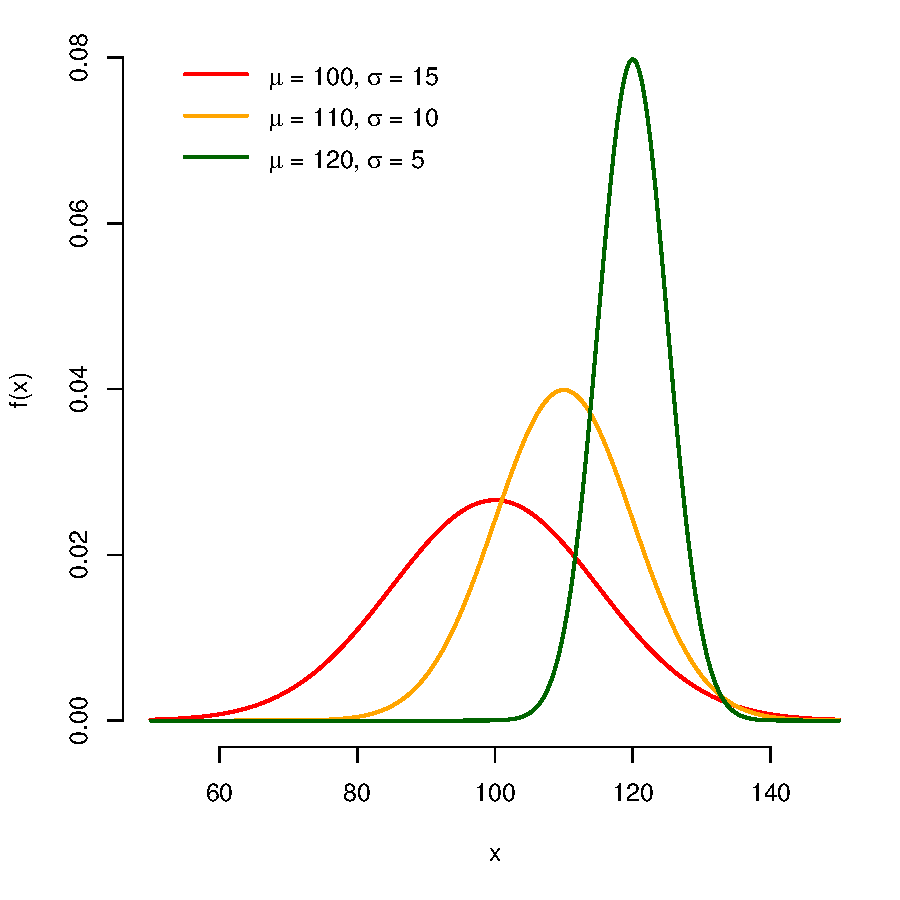
\includegraphics[width=0.7\linewidth]{img/ukazka-obr02.pdf}
\end{center}

TODO: add pictures, potentially a comparison of the old and new frontend.
\end{posterbox}

\begin{posterbox}[column=1, name=result2, below=result1]{Backend plugins}

TODO: add some pictures of the plugin or the example (docking)?
\begin{center}
\begin{tabular}{lrr}
 & \textbf{SomeProgram} & \textbf{ThisThesis} \\
\hline
Process A & 50\% & 58\% \\
Time for A & 35 days & \textcolor{green!80!black}{35 seconds} \\
Process B & \textcolor{red}{15\%} & 55\% \\
Time for B & 1 day & 8 hours \\
Price & 66.6 EUR & free
\end{tabular}
\end{center}
\end{posterbox}

\begin{posterbox}[column=1, name=result3, below=result2, headerColorOne=green!50!yellow, boxColorOne=green!10]{Main result}
\large\bfseries
\vspace{1ex}
\begin{center}
Program ThesisProgram solves the problem better than OtherProgram if X, and faster if Y.
\end{center}
\vspace{.5ex}
\end{posterbox}

\begin{posterbox}[column=1, name=conclusion, below=result3, bottomaligned=tech]{Source codes \& Contact}

Thesis supervisor: \textbf{doc. RNDr. David Hoksza, Ph.D.}, Department of Software Engineering

GitHub repository: \textbf{https://github.com/cusbg/prankweb}

Running instance: \textbf{https://prankweb.cz}


TODO: maybe add a QR code with the link to the repository or the running instance.
TODO: use the cusbg or mine?
\end{posterbox}

\end{poster}
\end{document}
